%%%%%%%%%%%%%%%%%%%%%%% file template.tex %%%%%%%%%%%%%%%%%%%%%%%%%
%
% This is a template file for Web of Conferences Journal
%
% Copy it to a new file with a new name and use it as the basis
% for your article
%
%%%%%%%%%%%%%%%%%%%%%%%%%% EDP Science %%%%%%%%%%%%%%%%%%%%%%%%%%%%
%
%%%\documentclass[option comma separated list]{webofc}
%%% Important option:
%%% "epj" for EPJ Web of Conferences Journal
\documentclass[epj]{webofc}
\usepackage[varg]{txfonts}   % Web of Conferences font
%
% Put here some packages required or/and some personal commands
%
%
\wocname{EPJ Web of Conferences}
%
\woctitle{ICNFP 2016}
%
%
%% Your personal definitions go here
\newcommand{\pt}{$p_{T}$}
\begin{document}
%
\selectlanguage{english}
\title{Search for new physics beyond the Standard Model in final states with jets and
  leptons+jets at CMS}
%
% subtitle (optional, strongly discouraged)
%
%%%\subtitle{Do you have a subtitle?\\ If so, write it here}

\author{Francesco
  Santanastasio\inst{1}\fnsep\thanks{\email{francesco.santanastasio@cern.ch}}
  on behalf of the CMS collaboration
        % etc.
}

\institute{Sapienza, University of Rome and INFN Rome 
}

\abstract{%
  Searches for new physics beyond the Standard Model
  performed by the CMS experiment in final states with
  jets and leptons+jets are presented. The document focuses on
  a selection of recent results from searches for heavy dijet resonances,
  leptoquarks, and heavy majorana neutrinos using proton-proton
  collision data at both $\sqrt{s}=$8 and 13 TeV.
  The novel CMS datascouting technique, used to probe the low-mass region in hadronic final
  states, is introduced and results from a Run1 analysis are shown.
  Two searches in the electrons+jets final states showing an excess
  of events in Run1 data are also discussed.
}
%
\maketitle
%
\section{Introduction}
\label{intro}
Searches for new physics beyond the Standard Model performed 
by the CMS experiment at the CERN LHC are presented in these conference proceedings.
A selection of searches in final states with jets and leptons+jets is
shown\footnote{The complete list of
publications and preliminary results on these subject are available 
in the CMS public web pages~\cite{EXOpages}.}. Results are obtained using proton-proton collision data 
collected in Run1 (2012) at $\sqrt{s}=8$~TeV and Run2 (2015) at $\sqrt{s}=13$~TeV.
Section~\ref{dijet} presents results of the search for dijet
resonances at high-mass using 2015 Run2 data and results 
of the low-mass analysis with the Run1 {\it data scouting} technique. 
Section~\ref{LQ} reports the results from searches for leptoquarks at
$\sqrt{s}=13$~TeV. In Section~\ref{excess} a few interesting excesses
of events in data observed in the Run1 searches for leptoquarks and
heavy majorana neutrinos are discussed. Finally the future prospects for
these searches are presented in Section~\ref{future}.

\section{Dijet resonances}
\label{dijet}
The search for new resonances decaying to pairs of jets is among the
most important ones at LHC because any hypothetical new particle that
might be produced originates from the colliding protons and therefore
it must couple to quarks and/or gluons. 

The analysis strategy consists in reconstructing the invariant mass of
the dijet system ($\rm{m}_{\rm{jj}}$) and searching for a resonant peak in its
spectrum. Wide-jets
(corresponding to a jet cone size of $\Delta R =\sqrt{{\Delta\eta}^2+{\Delta\phi}^2}=1.1$) are used to reconstruct the
energy of the initial partons from the resonance decay. This algorithm
improves the energy resolution by collecting final state radiation
from the outgoing partons. Events used for the search are required to
have $\Delta \eta_{jj}=|\eta_{j1}-\eta_{j2}|<1.3$ reducing
significantly the QCD multijet background in t-channel with respect to
the s-channel process of resonance production.
The search is performed in two different dijet mass regions
depending on the trigger strategy used: high-mass 
($\rm{m}_{\rm{jj}}> 1 ~\rm{TeV}$) and low-mass ($500 ~\rm{GeV}
<\rm{m}_{\rm{jj}}<1 ~\rm{TeV}$). 

\subsection{High-mass dijet search}
The high-mass analysis uses events collected by standard hadronic
triggers employed in many CMS analyses. The trigger requires that
events have $H_T>800$ GeV, where $H_T$ is the scalar sum of all jets
with $p_T>$40 GeV reconstructed at high level trigger (HLT).
Offline events are required to pass a cut on the dijet mass at 
approximately $\rm{m}_{\rm{jj}}>1$ TeV for which the trigger is fully efficient
on events in data passing the final dijet selection.

Figure~\ref{dijetEventAndMass} (left) shows a display of the highest dijet-mass event passing the full
selection, recorded by CMS during 2015 data taking. The reconstructed invariant mass
of the dijet system is about 6 TeV. 
Figure~\ref{dijetEventAndMass} (right) shows the dijet mass spectrum in 2.4 fb$^{-1}$ of data
collected in 2015 at $\sqrt{s}=13$~TeV~\cite{Khachatryan:2015dcf}. The background is estimated
by fitting the data with a smoothly falling function. The
parametrization used is 
\begin{equation}
\frac{d\sigma}{d\rm{m}_{\rm{jj}}} = \frac{P_0 (1-x)^{P_1}}{x^{P_2+P_{3}ln(x)}}
\end{equation}
where $x=\rm{m}_{\rm{jj}} / \sqrt{s}$. 
This function models well the QCD multijet simulation and the data
and it has been successfully employed in previous searches at hadron
colliders at different $\sqrt{s}$ values.
%
\begin{figure}[h]
\centering
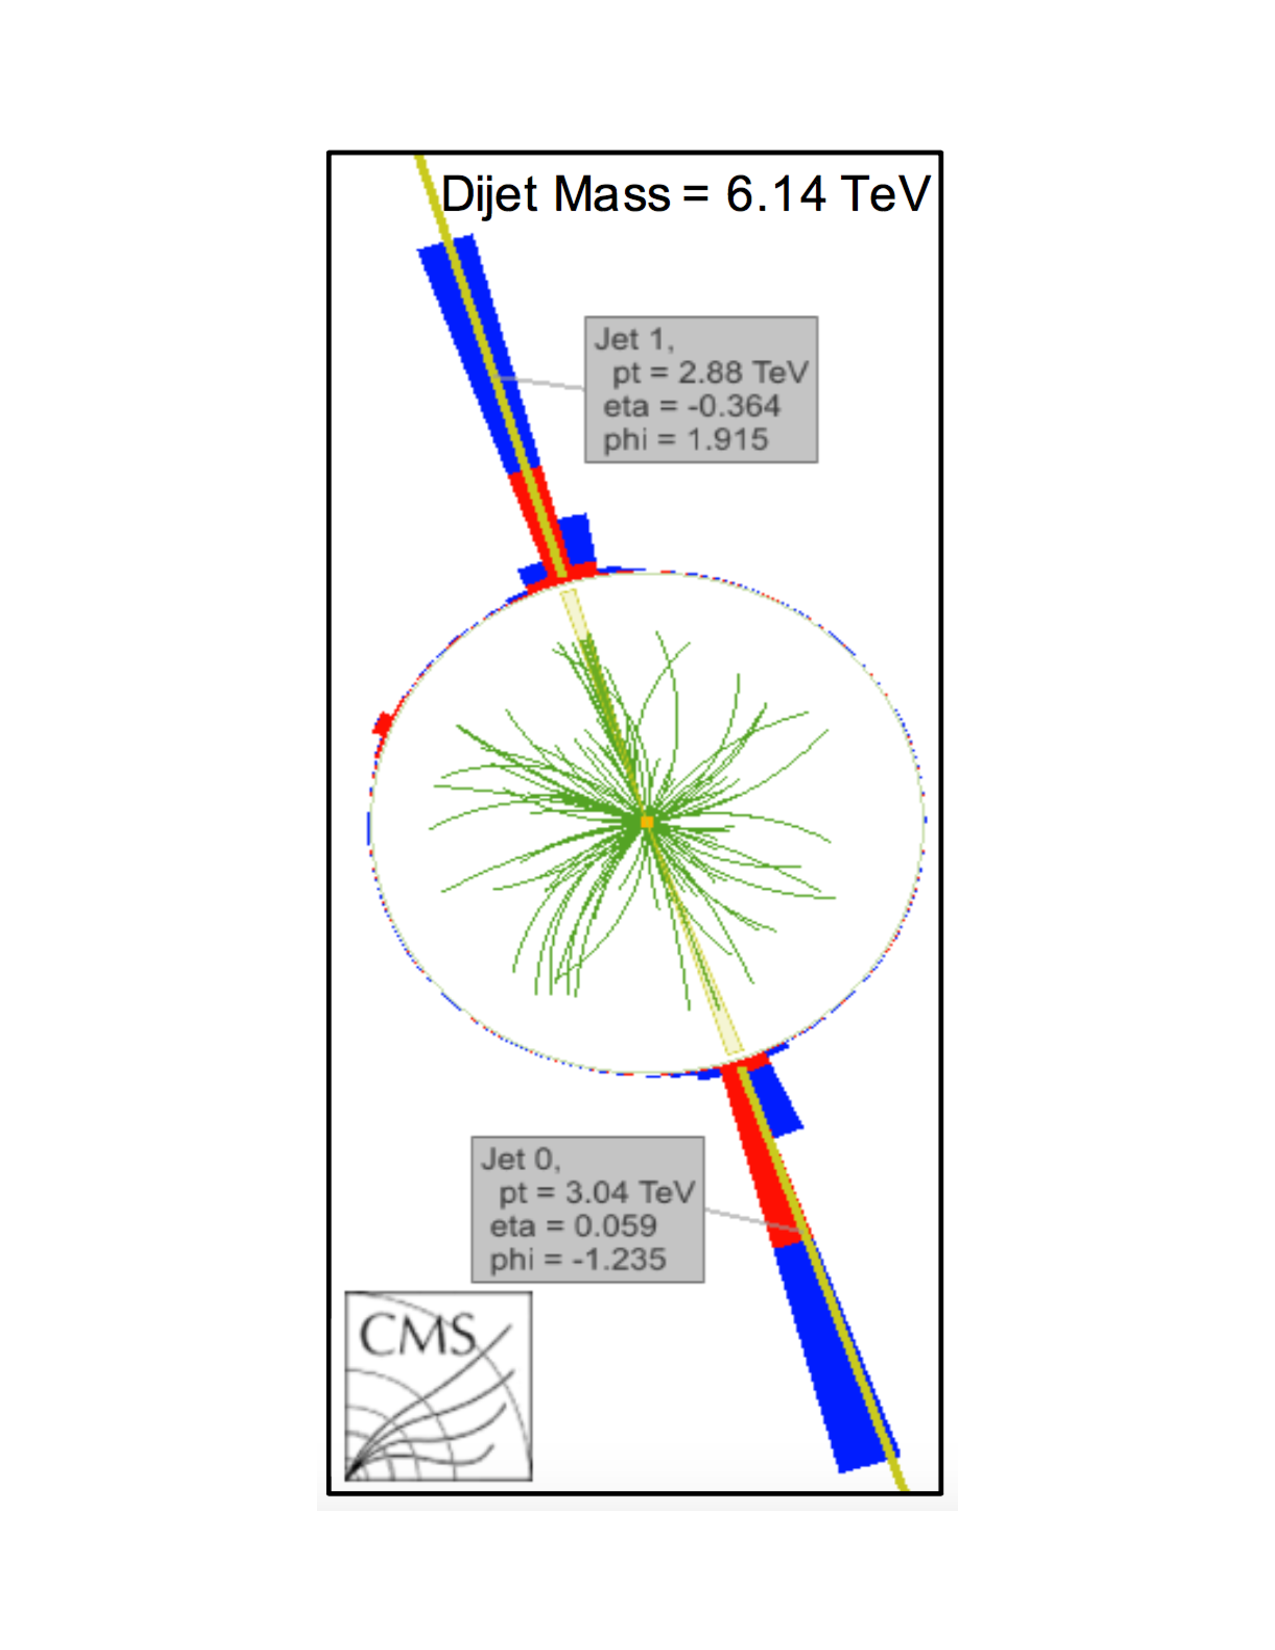
\includegraphics[width=6cm,clip]{CMS-EXO-15-001_Figure-aux_009.pdf}
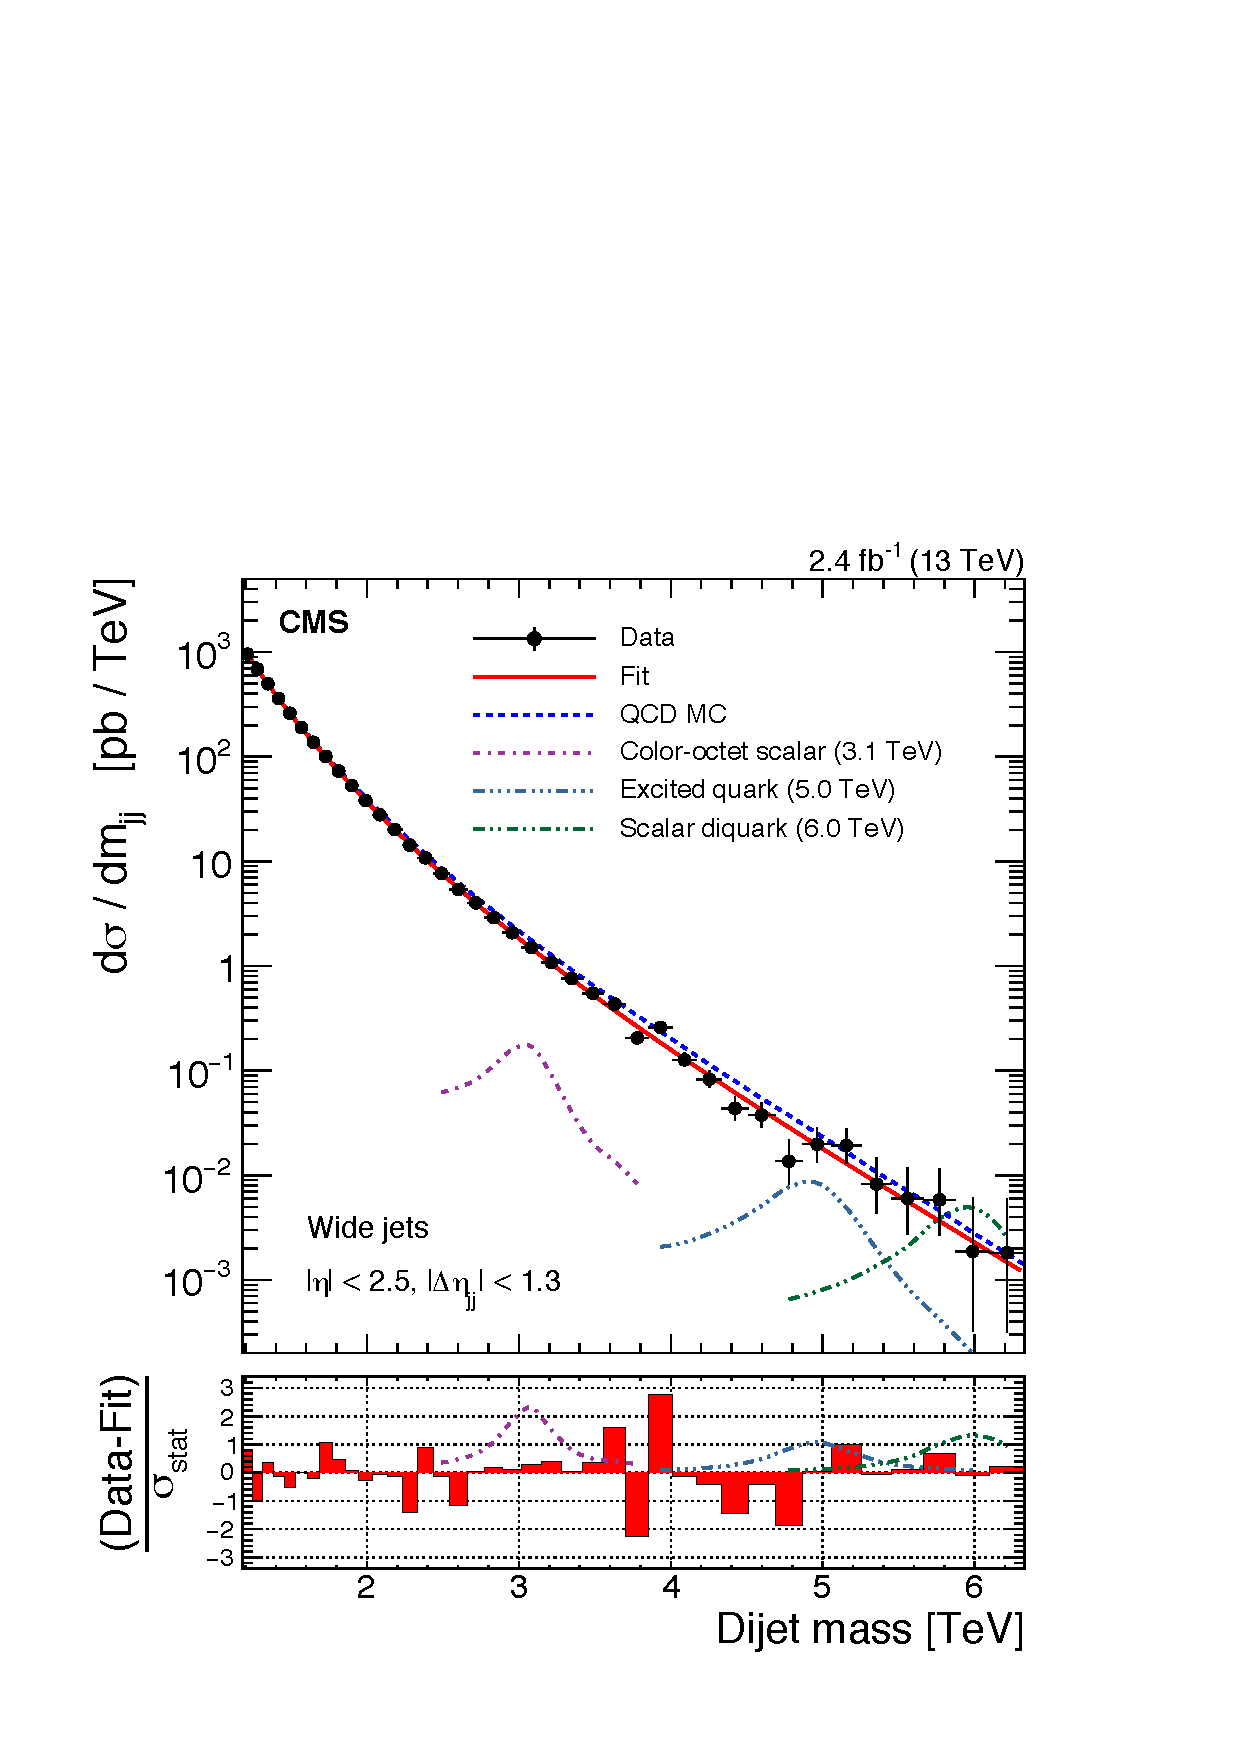
\includegraphics[width=6cm,clip]{CMS-EXO-15-001_Figure_001.pdf}
\caption{Left: Display of the event with the highest dijet mass (6.14 TeV)
  after the full selection. The transverse view with respect to the
  beam axis is shown. The kinematic quantities of the two wide jets
  are reported. Right: Dijet mass spectrum (points) compared to a fitted
  parameterization (solid curve) and to the prediction 
of the PYTHIA8 QCD MC event generator including simulation of the
detector (dashed curve). The lower panel shows the difference between
the data and the fitted parametrization, divided by the statistical
uncertainties. The predicted distributions of narrow resonance signals
for three models, with resonance mass values corresponding to the
respective 95\% confidence level exclusion limit, are shown in both panels (dash-dotted curves).}
\label{dijetEventAndMass}       % Give a unique label
\end{figure}
%
No sign of new resonances is observed in the dijet mass spectrum, and
95\% confidence level (CL) upper limits are set on the resonance 
production cross section ($\sigma$) time branching ratio to dijet
($BR$) times acceptance ($A$) as a function of the hypothesized
resonance mass. The limits are reported in Figure~\ref{dijetLimits} (left) for
different final states (quark-quark, quark-gluon, gluon-gluon
depending on the resonance decay products). The upper limits on
$\sigma \times BR \times A$ are compared to theoretical predictions
for several new physics models including strongly coupled
resonances (such as string resonances, excited quarks, axigluons, etc.) and
weakly coupled resonances (such as Z' and W' bosons and Randall-Sundrum Gravitons), covering a
wide range of cross sections to which this analysis is
sensitive. Lower limits are set on the mass of these resonances 
as summarized in Figure~\ref{dijetLimits} (right). The limits of this analysis 
significantly exceed the ones from the previous Run1 search thanks 
to the increased center-of-mass energy in Run2.  
%
\begin{figure}[h]
\centering
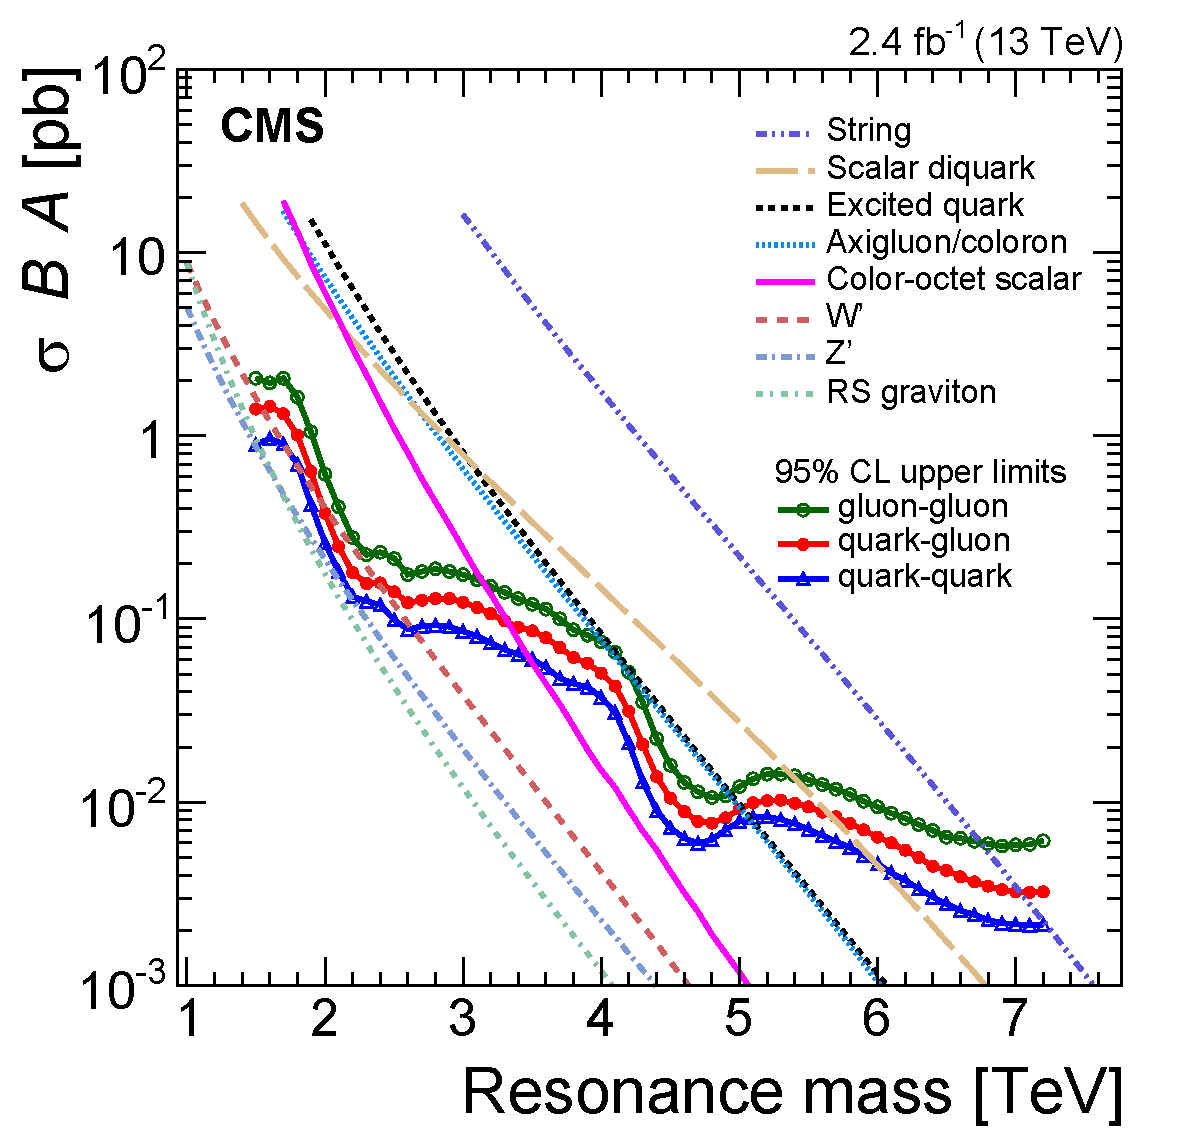
\includegraphics[width=7cm,clip]{CMS-EXO-15-001_Figure_003-d.pdf}
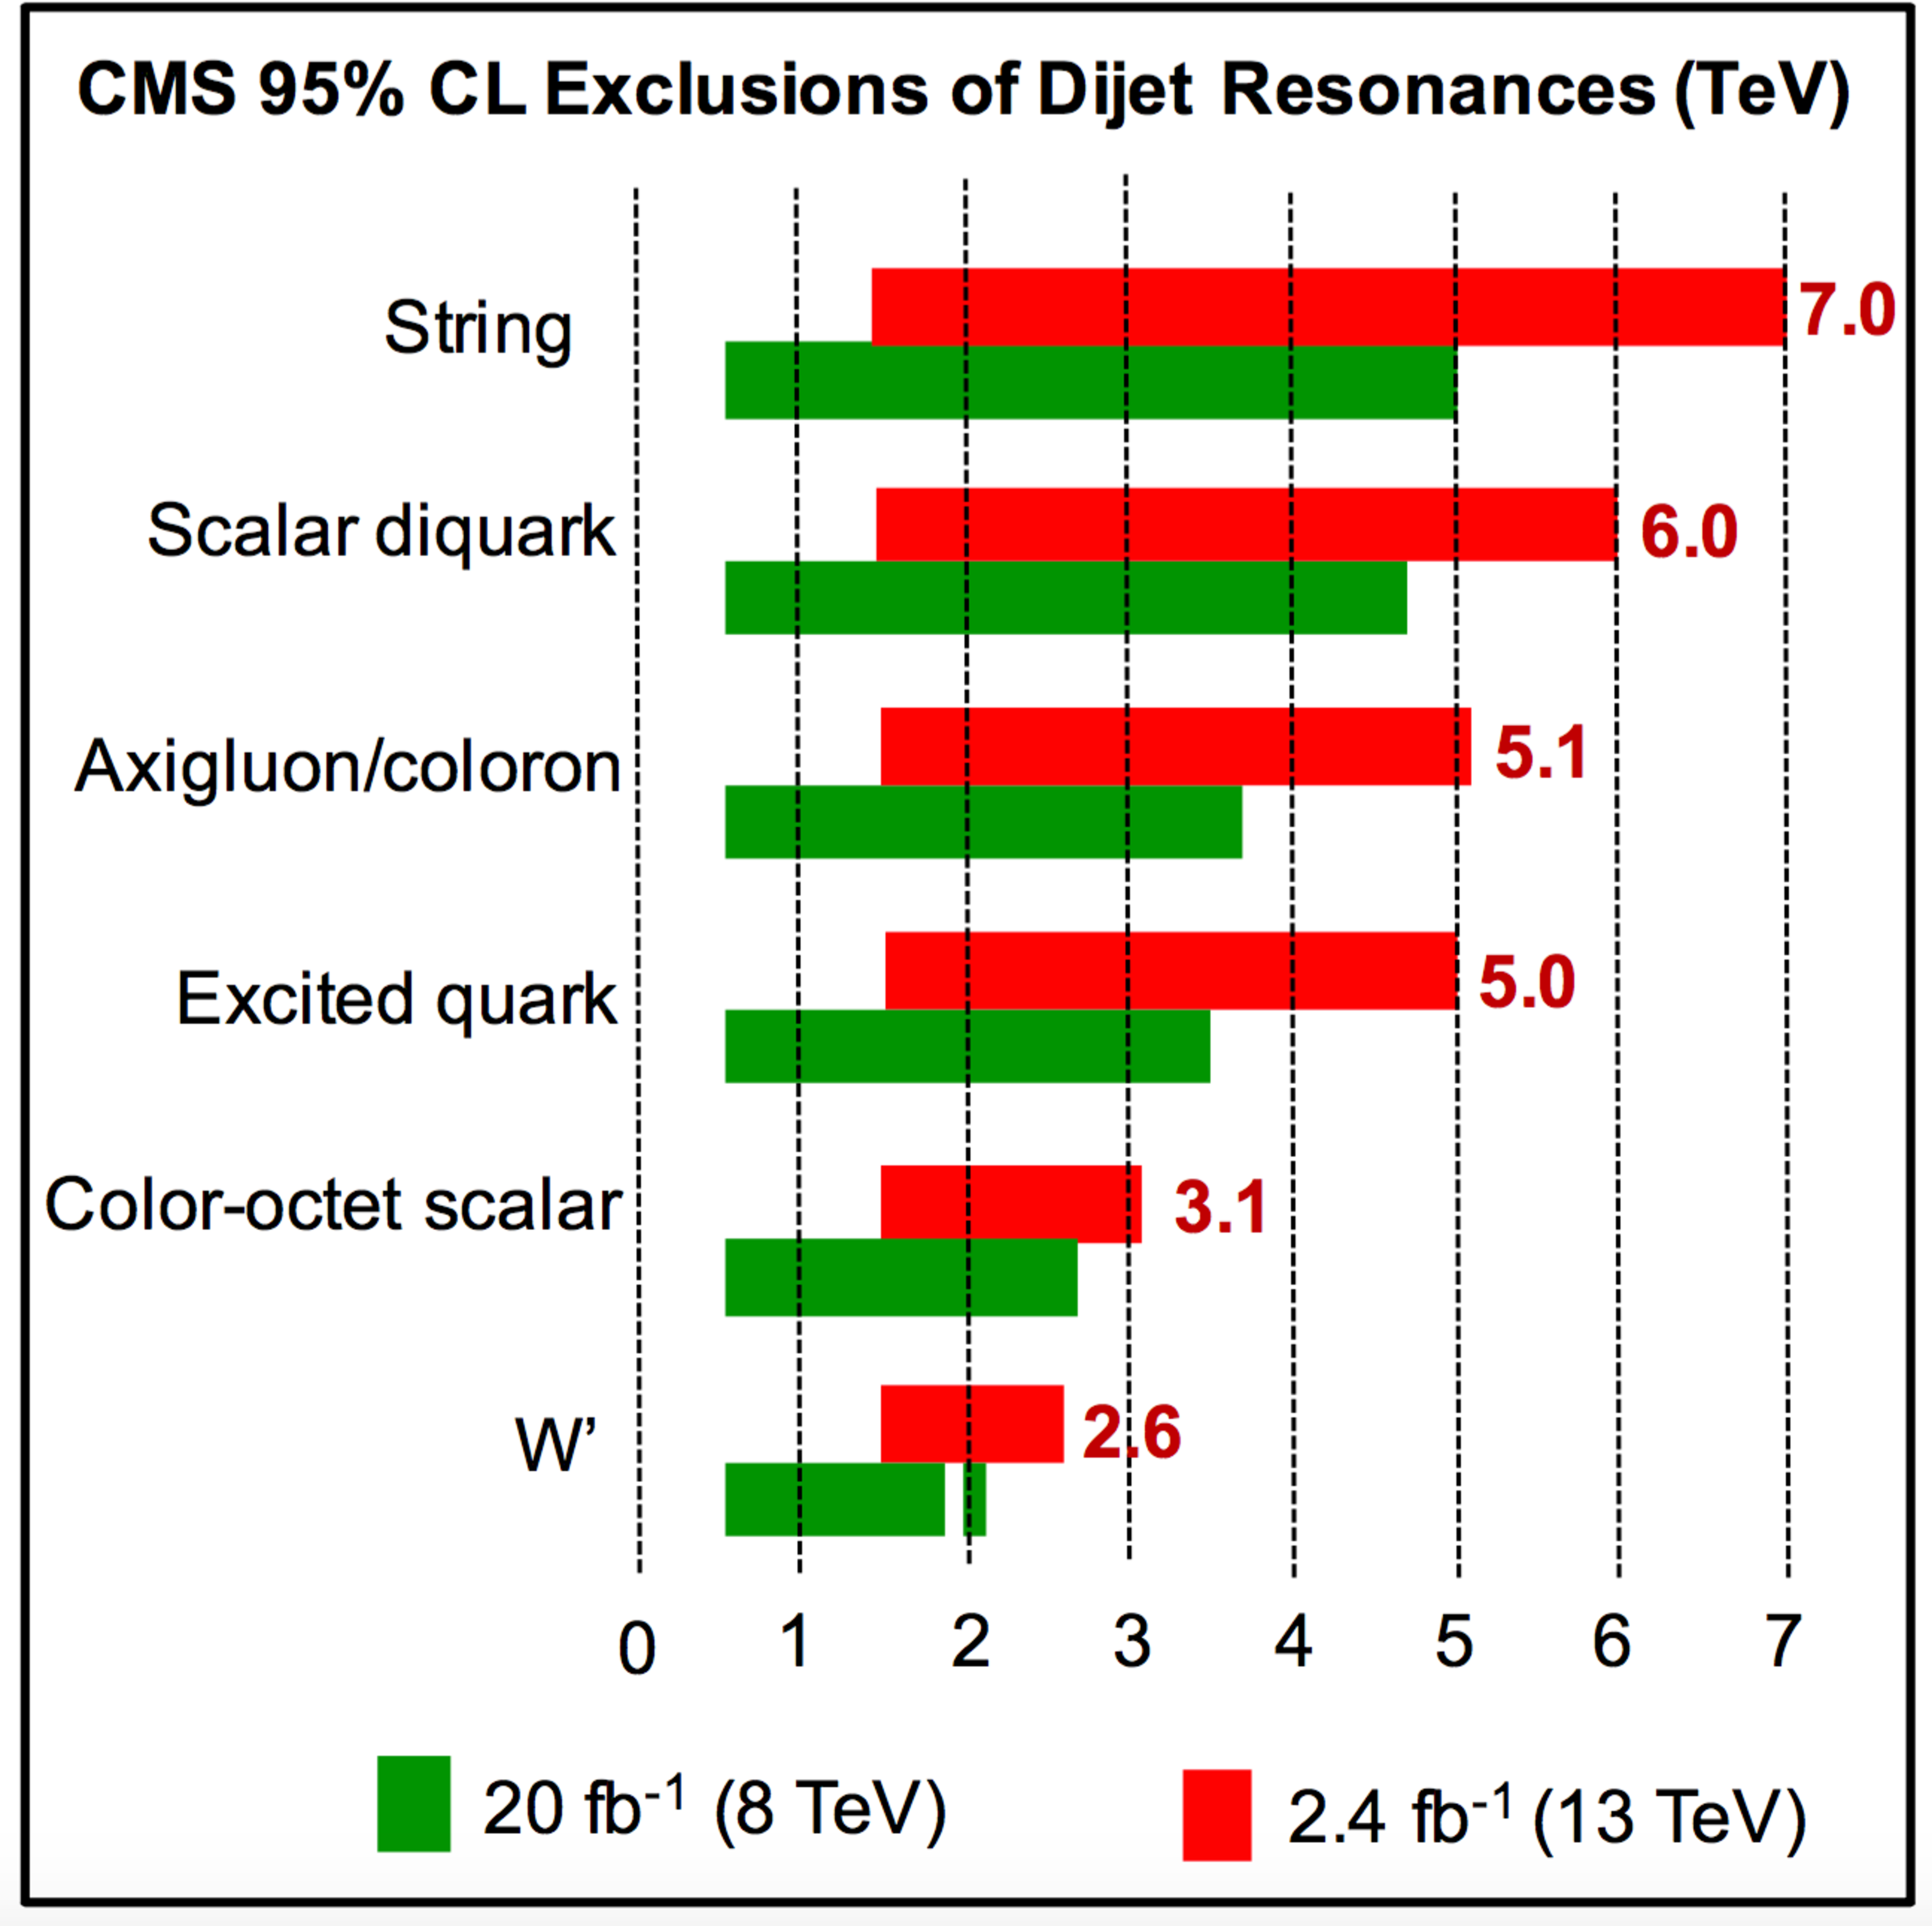
\includegraphics[width=6cm,clip]{CMS-EXO-15-001_Figure-aux_013.png}
\caption{Left: The observed 95\% CL upper limits on the product of the
  cross section, branching fraction, and acceptance for quark-quark,
  quark-gluon, gluon-gluon type dijet resonances.  The limits are
  compared to the predicted cross sections of  several resonance
  models. Right: Observed 95\%CL lower limits on resonance mass
  for the listed models obtained by the CMS experiment in Run 1
  (green) and Run 2 (red) analyses.}
\label{dijetLimits}       % Give a unique label
\end{figure}
%

\subsection{Low-mass dijet search with data scouting}
It is important to extend the dijet search in the mass region below 1
TeV in order to probe hypothetical hadronic resonances with small
couplings to quarks and gluons that similar searches performed at previous
colliders could not find yet. The main experimental difficulties at LHC originate
from the large cross section of multijet events at low dijet mass 
and the finite computing resources for processing and storing these
data. To solve this issue, a new technique known as 
{\it data scouting} was first proposed by CMS in 2011~\cite{CMS:2012cza}. 
This technique, by significantly reducing the event size
compared to the standard CMS data stream (about a factor 100), enabled CMS to relax the
trigger thresholds and record fully hadronic events at a rate of few
KHz to extend the search in the sub-TeV mass region. With this approach, the
analysis is performed using jets reconstructed online in the CMS
trigger computing farm. 

This novel research strategy was fully integrated in the CMS physics program in
2012~\cite{CMS:2012ooa} allowing to collect data corresponding to almost 19 $\rm{fb}^{-1}$ of
integrated luminosity at $\sqrt{s}=8$~TeV in the sub-TeV dijet mass
region. The new trigger allows to go down to 400 GeV in dijet mass. 
The offline analysis strategy used for the high-mass analysis is also employed
in this low-mass search. Figure~\ref{dijetScouting} (left) shows the dijet mass spectrum in scouting data in the
region between 400 and 1900 GeV. No sign of new resonances in observed and upper limits on 
$\sigma \times BR \times A$ are set as a function of the resonance
mass. The analysis results has been published on the PRL journal in 2016~\cite{Khachatryan:2016ecr}. 

It is interesting to compare the limits of this search with those obtained 
by previous experiments at hadronic colliders with different 
center-of-mass energies. This can be done assuming a common 
theoretical model of a new resonance Z' that decays to a
pair of quarks as described in Ref.~\cite{Dobrescu:2013coa}. This simplified model is characterized 
by only two free parameters: the resonance mass $M_{Z'}$ and the 
coupling $g_B$ of the resonance to the quarks. The upper 
limits on signal cross section can be translated into limits in the
coupling vs mass plane as shown in Figure~\ref{dijetScouting} (right). The CMS dijet analysis
with data scouting extends the search below 1 TeV and provides, at 
the time of the publication, the most stringent limits to date in the
region between 500 and 800 GeV. 
In the region below 500 GeV the best limits still come from 
CDF and UA2 experiments. ATLAS and CMS have initiated recently a
physics program targeting the mass region below 500 GeV using various
techniques that exploit the emission of initial state radiation
(quarks/gluons or photons) to trigger these events. 
%These results
%including the updates of the CMS analysis with data scouting at $\sqrt{s}=13$~TeV, 
%will be presented at the ICHEP conference in Summer 2016.
%
\begin{figure}[h]
\centering
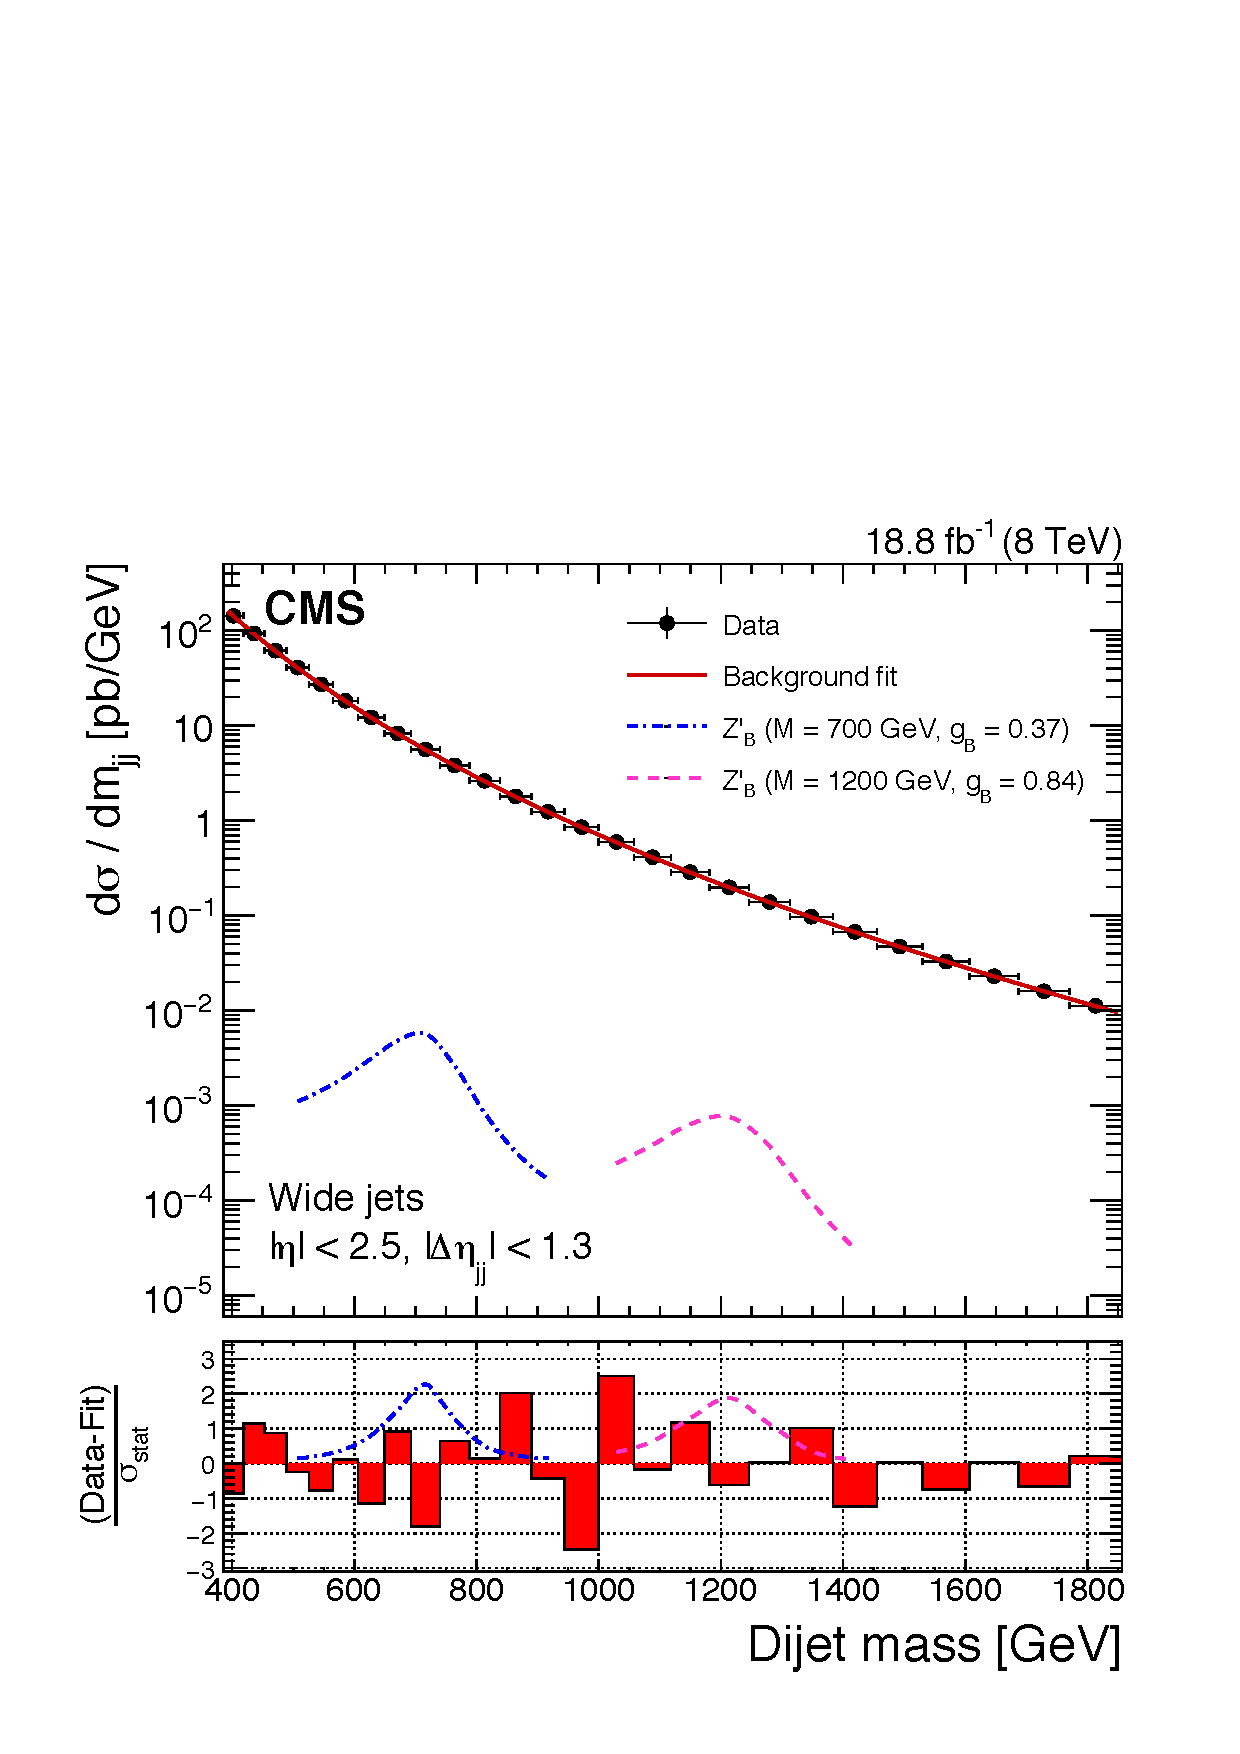
\includegraphics[width=5cm,clip]{CMS-EXO-14-005_Figure_001.pdf}
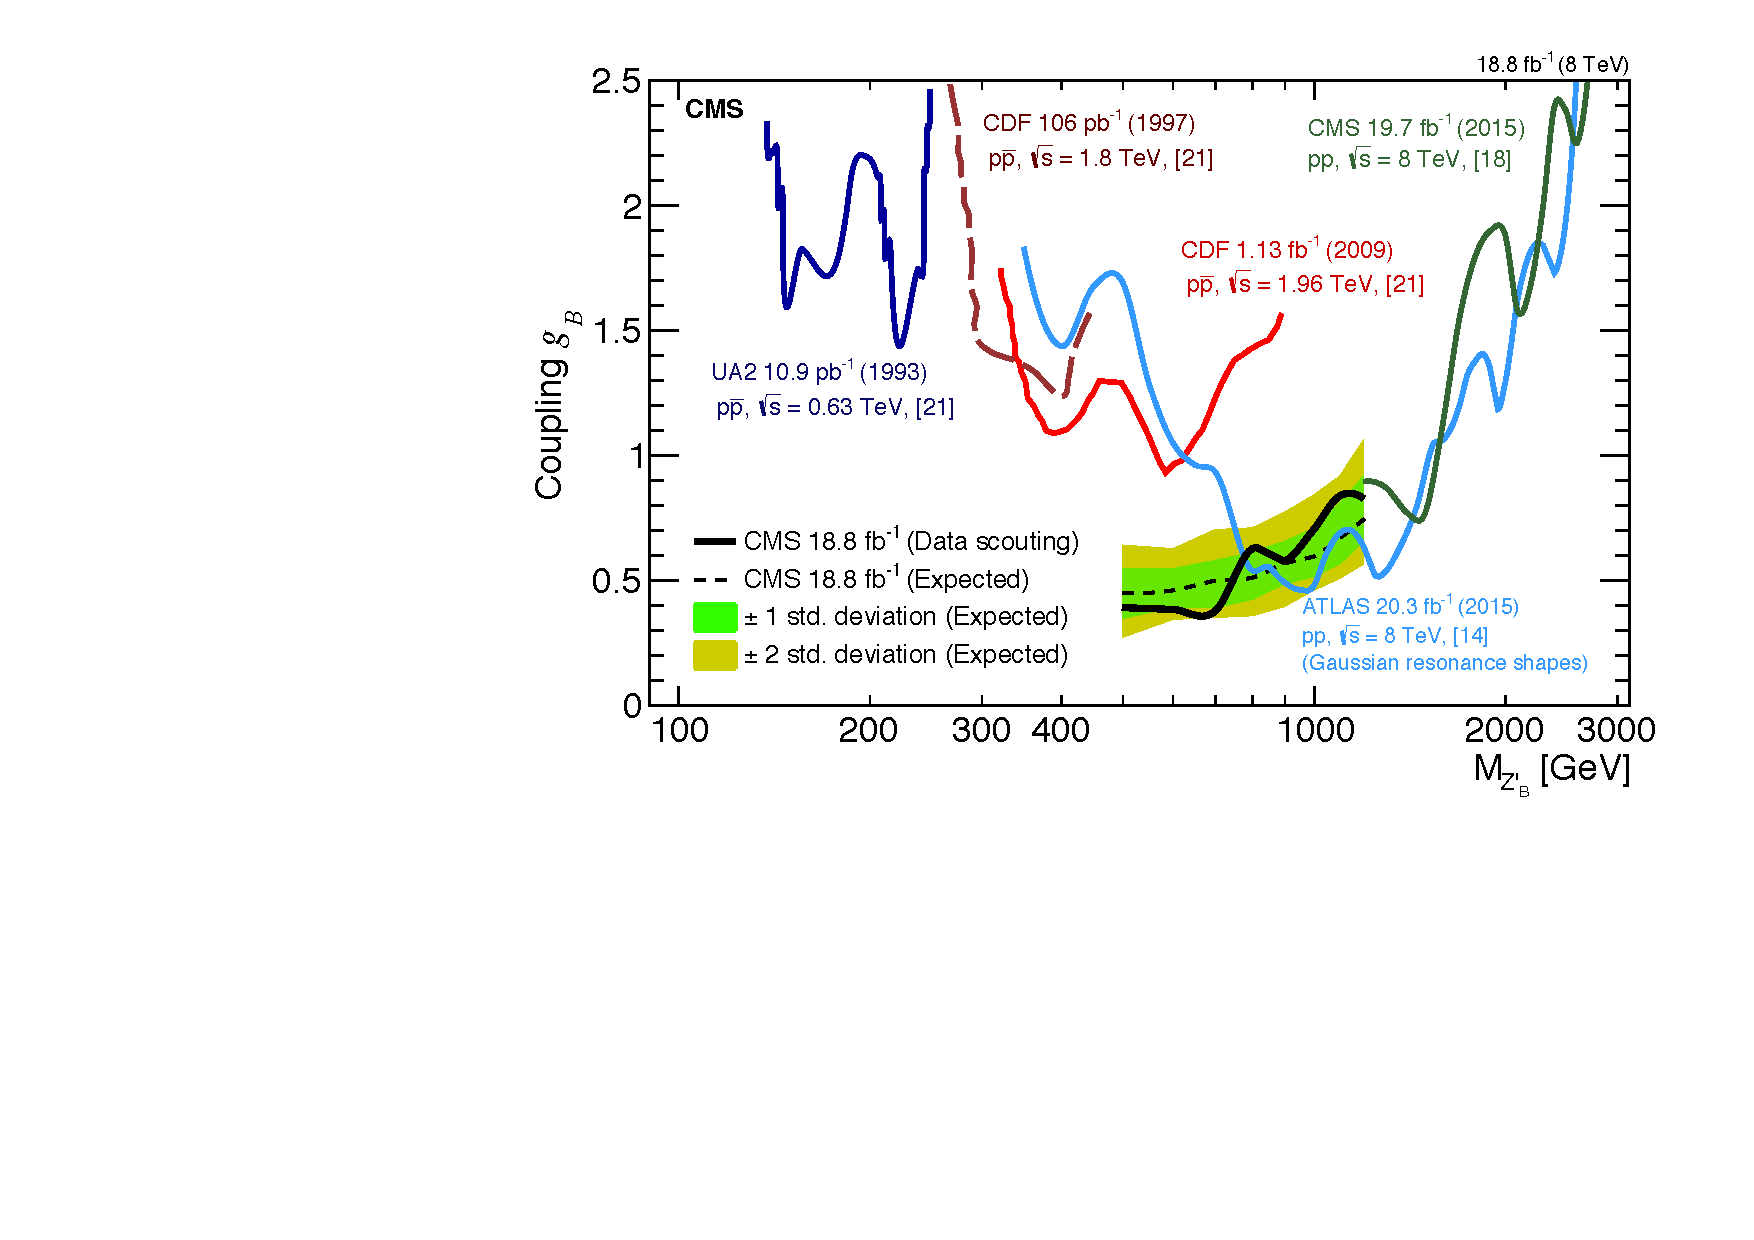
\includegraphics[width=9cm,clip]{CMS-EXO-14-005_Figure_004.pdf}
\caption{Left:  Dijet mass spectrum using data scouting (points) compared to a fitted
  parameterization (solid curve). The bottom panel compares the data
  and the fit result, normalized by the statistical uncertainty in the
  data, for each bin. The predicted distributions of narrow resonance
  signals for a hypothetical leptophobic resonance Z' with two
  different mass and coupling values are shown in both panels
 (dash-dotted curves). This dijet mass distribution complements that 
observed in the high-mass analysis. Right: Observed 95\% CL upper
limits on the coupling $g_B$ of the Z' resonance as a function of its
mass. The results are compared to those obtained with similar searches
at different collider energies.}
\label{dijetScouting}       % Give a unique label
\end{figure}
%

\clearpage

\section{Leptoquarks}
\label{LQ}

The Standard Model contains hints that the lepton and quark sectors
are related by a fundamental symmetry. Many beyond the Standard Model
theories (such as grand unified theories, composite models,
technicolor, SUSY RPV, and others) include such a symmetry, 
and predict the existence of new massive bosons called leptoquarks (LQ).
Leptoquarks can have spin 0 or 1, are coloured particles, have
fractional electric charge, and carry both baryon and lepton number.
In order to avoid proton decay, baryon and lepton numbers must be
conserved separately. In addition constrains from rare decays involving
flavour-changing-neutral-currents suggests that LQs should only couple
with leptons and quarks within the same generation. 

In the simplest
case, the model parameters are three: the mass of the LQ ($M_{LQ}$), the branching
ratio of the LQ decay into charged lepton and quark ($\beta$), and the 
LQ-lepton-quark coupling ($\lambda$). The branching ratio of the LQ
decay into neutrino and quark is $1-\beta$. At LHC, LQs can be produced singly
or in pairs. The pair production, which happens mainly via gluon-gluon
fusion, is particularly interesting because it does not depend on the
unknown coupling $\lambda$. The pair production cross section depends on 
the strong coupling and it is calculated at next-to-leading order.

Depending on the value of the parameter $\beta$ different decay channels
are possible from the pair production of LQs. They differ for the
branching ratio ($BR$) and the observed final state, thus producing a
wide range of experimental signatures: 
\begin{itemize}
\item $\ell\ell jj$ channel, $BR=\beta^2$, two charged leptons plus two jets;
\item $\ell\nu jj$ channel, $BR=2\beta(1-\beta)$, one charged leptons,
  missing transverse energy (MET) plus two jets;
\item $\nu\nu jj$ channel, $BR=(1-\beta)^2$, two jets plus MET.
\end{itemize}
Feynman diagrams for the different final states are shown in Figure~\ref{LQdiagram}.
%
\begin{figure}[h]
\centering
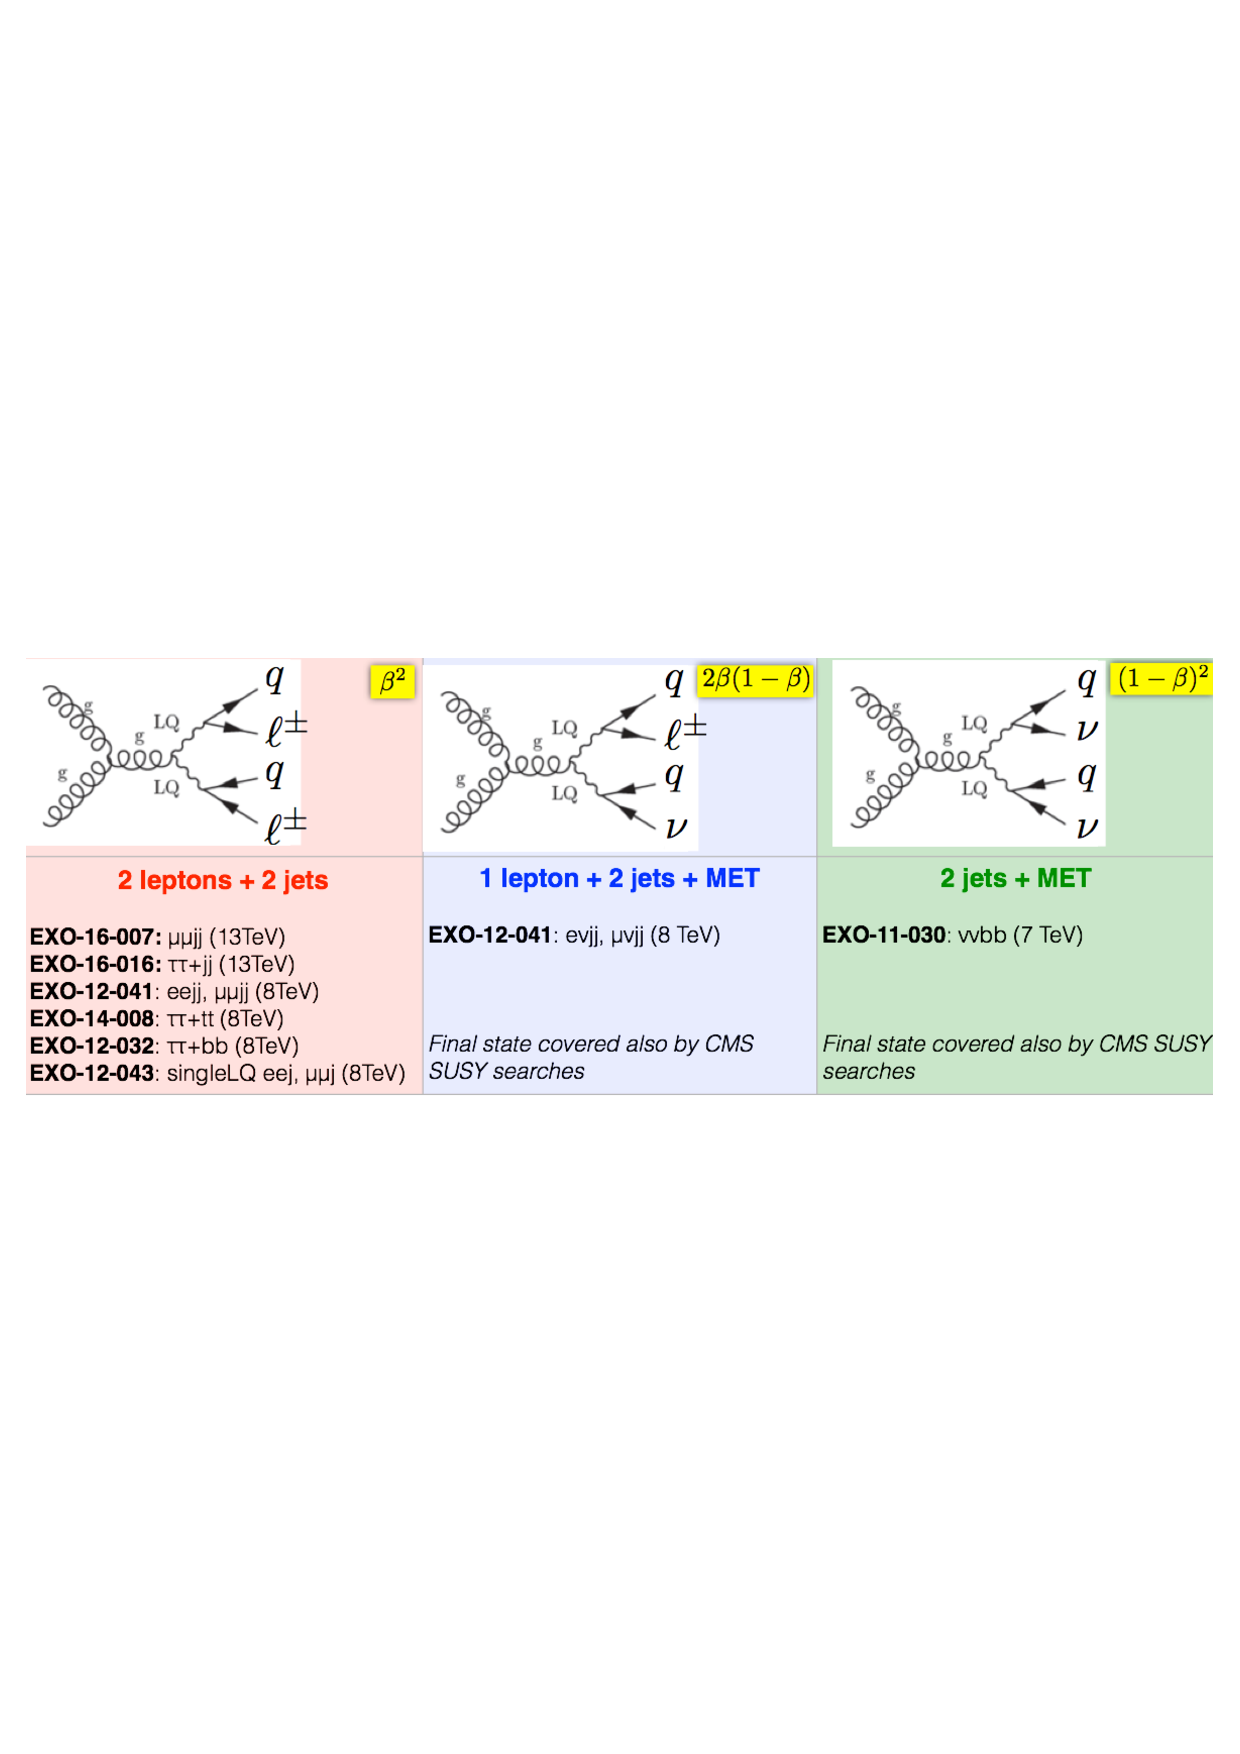
\includegraphics[width=13cm,clip]{LQdiagram.pdf}
\caption{Feynman diagrams for different final states in LQ pair
 production processes. The labels {\sc EXO-XX-YYY} indicates the identifier
of the CMS publications or preliminary results describing the most recent 
searches in the corresponding channel~\cite{EXOpages}.}
\label{LQdiagram}       % Give a unique label
\end{figure}
%

The most recent searches for LQ at CMS have been performed using about 2 fb$^{-1}$ of 
$\sqrt{s}=13$~TeV data collected in 2015.

A search for second generation LQs is
performed in final states with two muons and two jets~\cite{CMS:2016qhm}. The event
selection, optimized for each LQ mass hypothesis, is based on three
main kinematic observables: the di-muon invariant mass, the
$S_T=p_T(\mu_1)+p_T(\mu_2)+p_T(jet_1)+p_T(jet_2)$ variable, and the
lepton-jet mass $M^{min}_{\mu j}$ defined as the smaller of the two reconstructed
LQ masses which minimizes the LQ-LQ mass difference. In presence of a
signal, the $M^{min}_{\mu j}$ distribution would show a narrow peak in 
correspondence of the LQ mass, as shown in Figure~\ref{LQresults} (left). 

A search for third generation LQs is performed in final states with
two taus (with reconstructed hadronic decays) and two jets~\cite{CMS:2016xxl}.
The main physics observable to discriminate between signal and
background is the variable $S_T=p_T(\tau_1)+p_T(\tau_2)+p_T(jet_1)+p_T(jet_2)$
shown in Figure~\ref{LQresults} (right). 

No excess of events is observed in data in these searches and lower
limits are set on the mass of second and third generation LQs at 1150
GeV and 740 GeV, respectively, assuming $\beta=1$.
%
\begin{figure}[h]
\centering
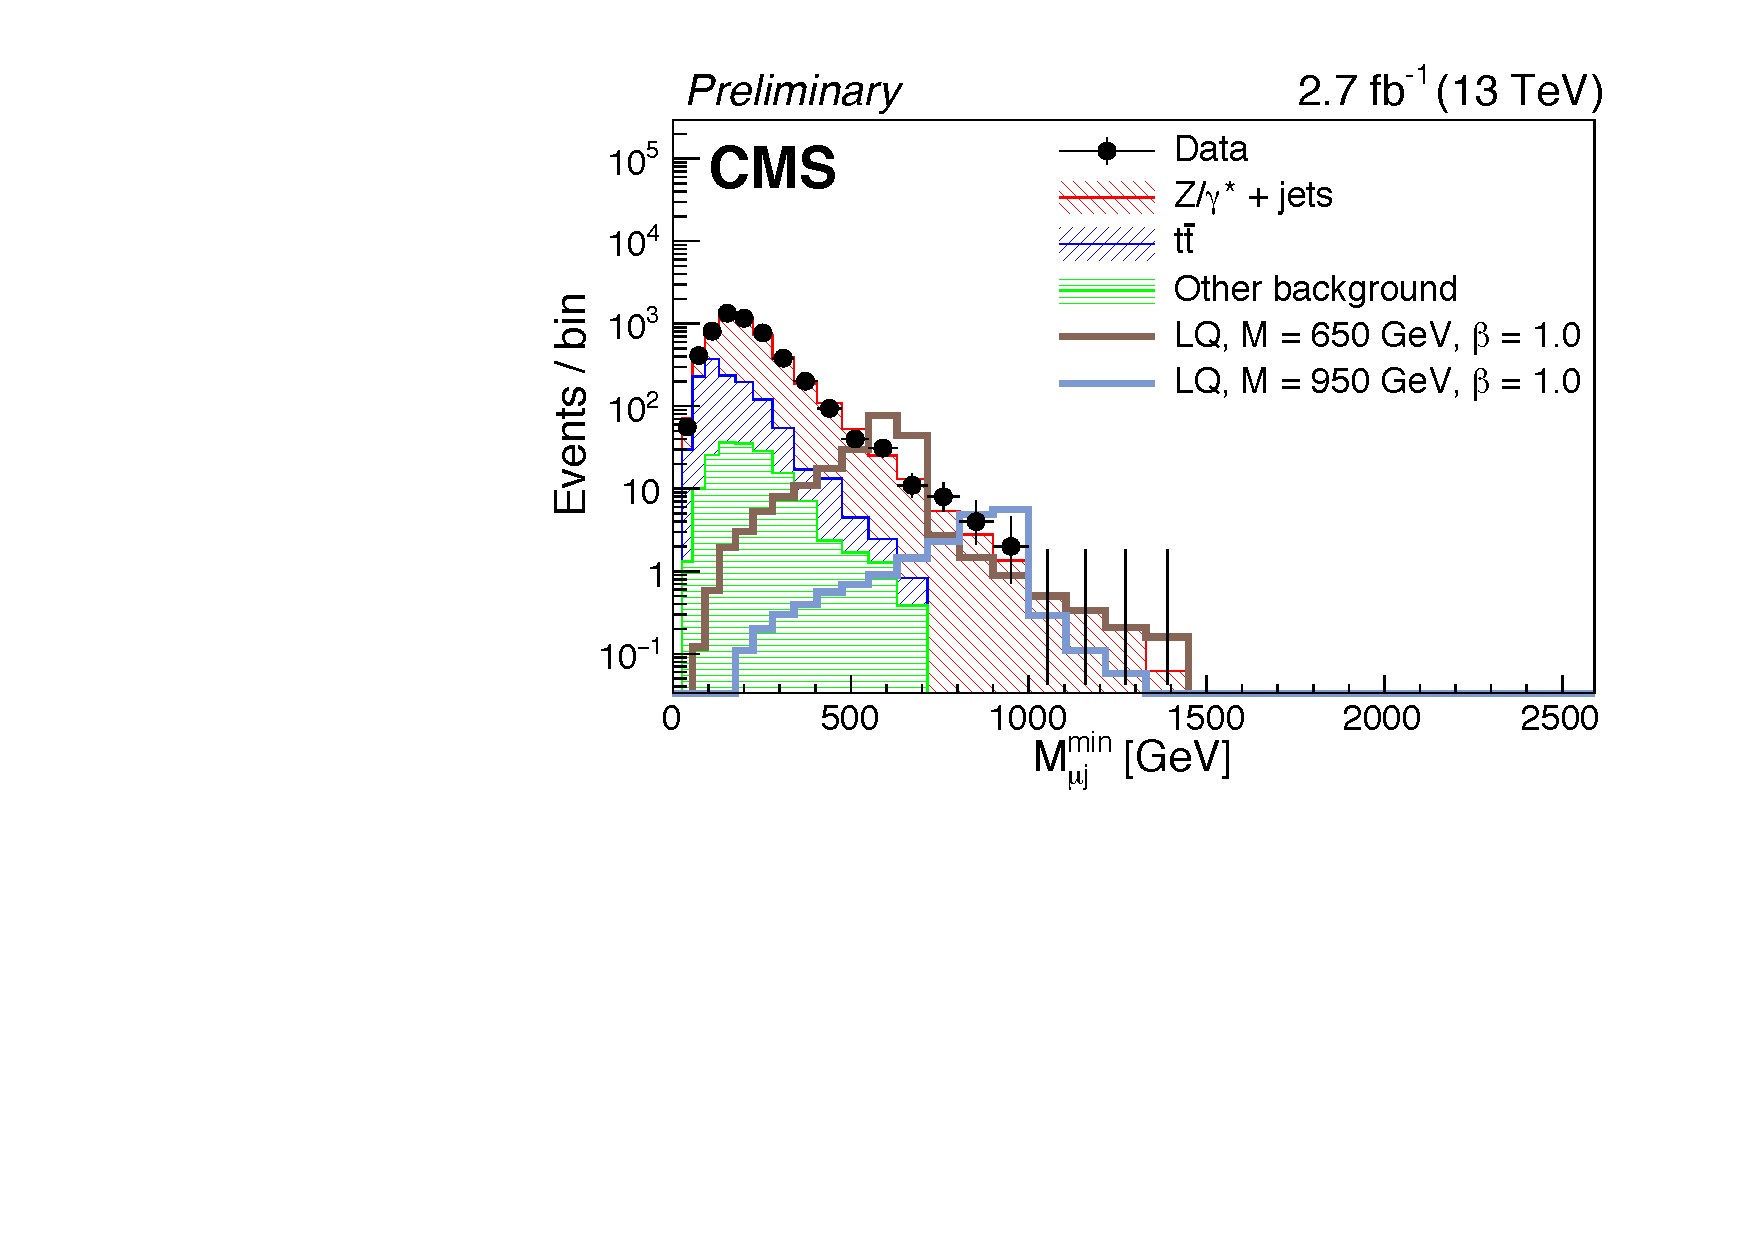
\includegraphics[width=7cm,clip]{CMS-PAS-EXO-16-007_Figure_002-c.pdf}
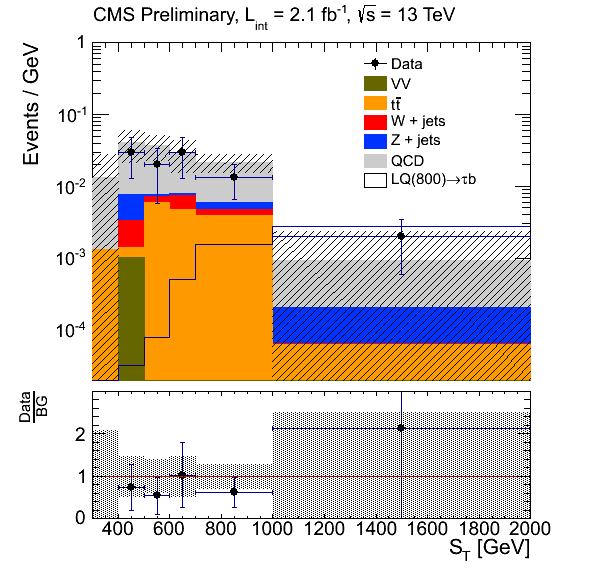
\includegraphics[width=6cm,clip]{CMS-PAS-EXO-16-016_Figure_002-b.png}
\caption{The $M^{min}_{\mu j}$ distribution in events with two muons and two
  jets (left). The $S_T$ distribution in events with two taus
  decaying hadronically and two jets (right). Distributions for the
  data, the background predictions, and the expected LQ signals are shown.}
\label{LQresults}       % Give a unique label
\end{figure}
%

\section{Excess of events in Run1 data}
\label{excess}

Searches for new physics in final states with leptons+jets have been
performed also in Run1 data at $\sqrt{s}=8$~TeV. Two of these searches
in final states with electrons and jets are particularly interesting
because they report an excess of events in data compared to
the background prediction.

\subsection{First generation leptoquarks}

A search for first generation leptoquarks in the $e\nu jj$ channel
have been performed with about 20 fb$^{-1}$ of data~\cite{Khachatryan:2015vaa}. The analysis is
designed as a counting experiment in a signal region defined by an
event selection optimized for each LQ mass hypothesis. The
reconstructed observables used in the selection to separate signal from background
are the electron-neutrino transverse mass, the variable $S_{T}=p_T(e_1)+MET+p_T(jet_1)+p_T(jet_2)$, 
and the electron-jet mass $M_{ej}$. Figure~\ref{LQ1} (left) shows the 
electron-jet mass distribution after a selection optimized for the
search of a LQ with 650 GeV mass. A broad excess of data events is visible 
above 600 GeV compared to the background expectation. This reflects also in the
upper limits on signal cross section times branching ratio shows in
Figure~\ref{LQ1} (right) in the same LQ mass region. The local significance of
the excess is 2.6 standard deviations. No excess is observed in the
$\mu\nu jj$ channel.
%
\begin{figure}[h]
\centering
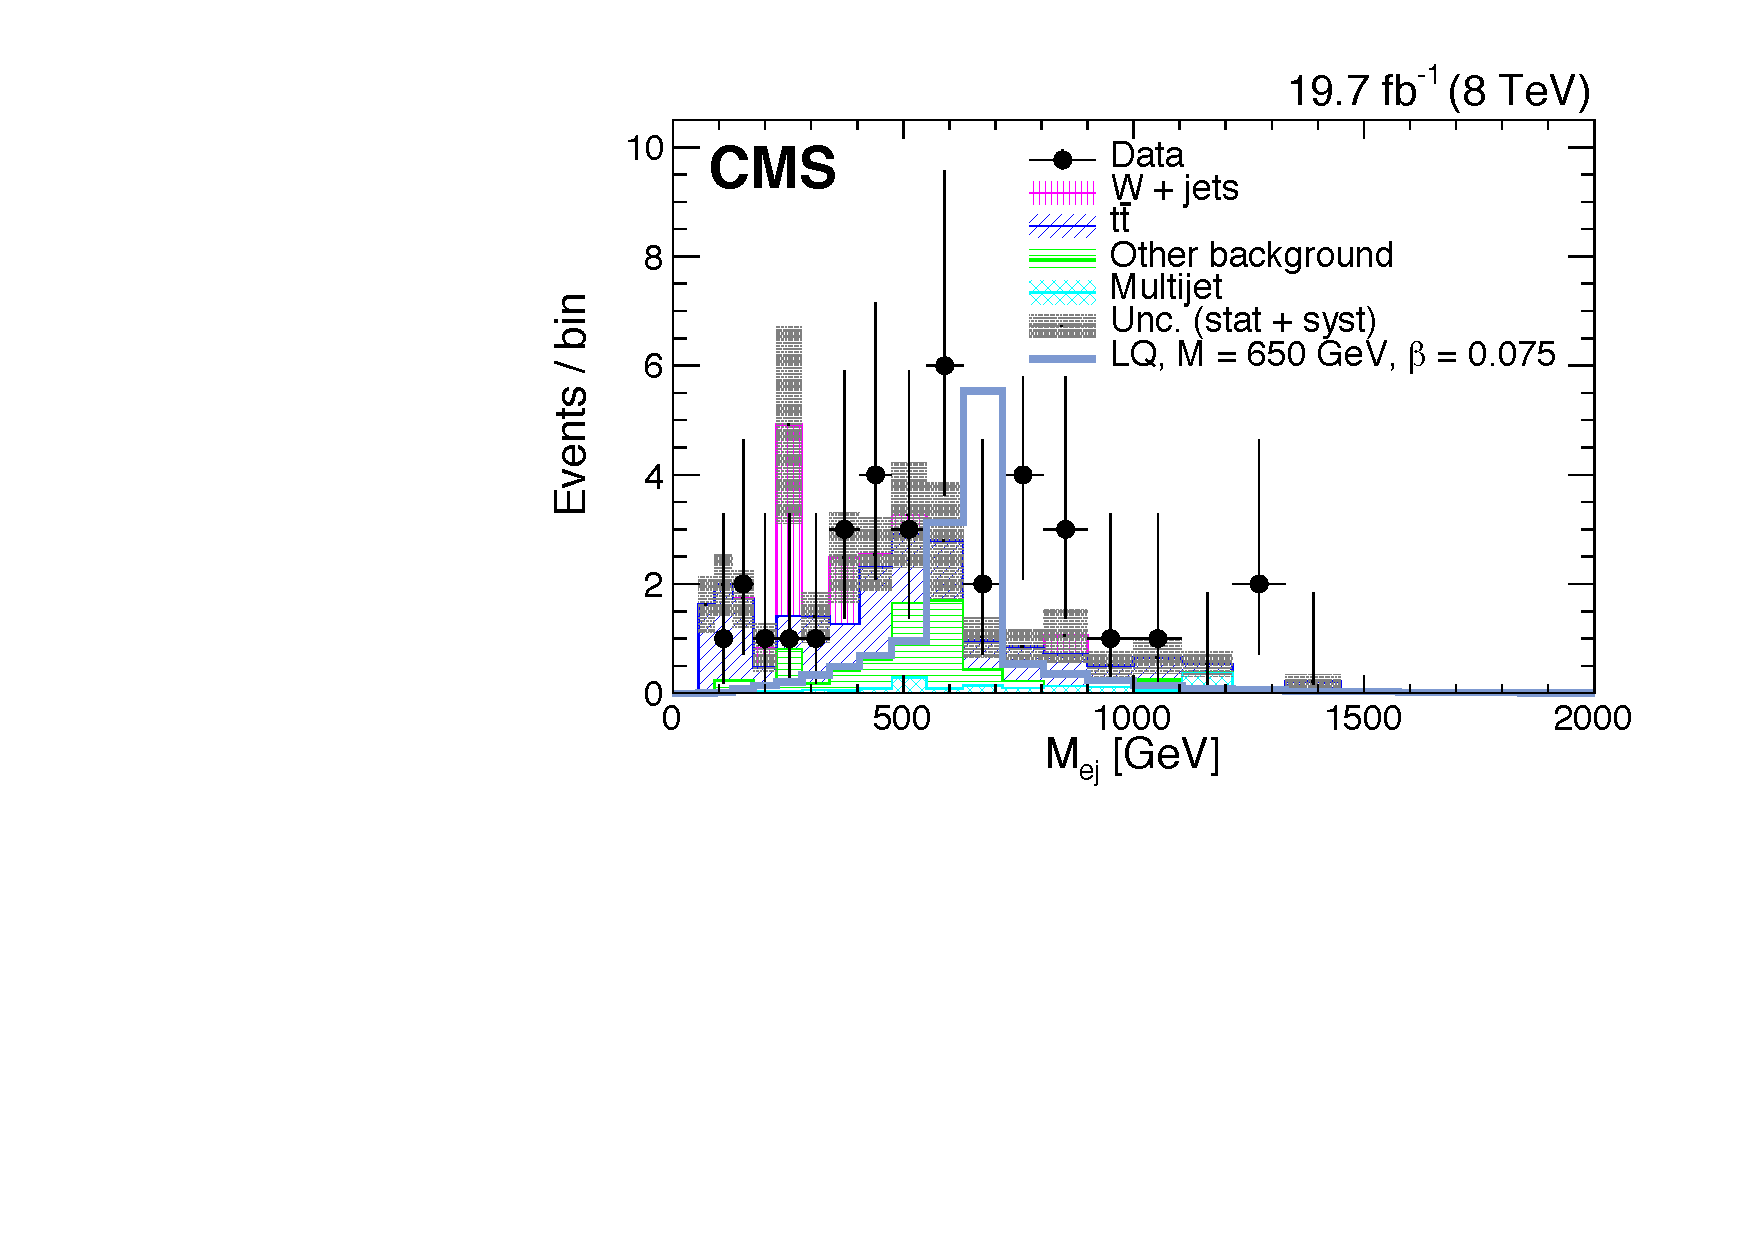
\includegraphics[width=8cm,clip]{CMS-EXO-12-041_Figure_009-b.pdf}
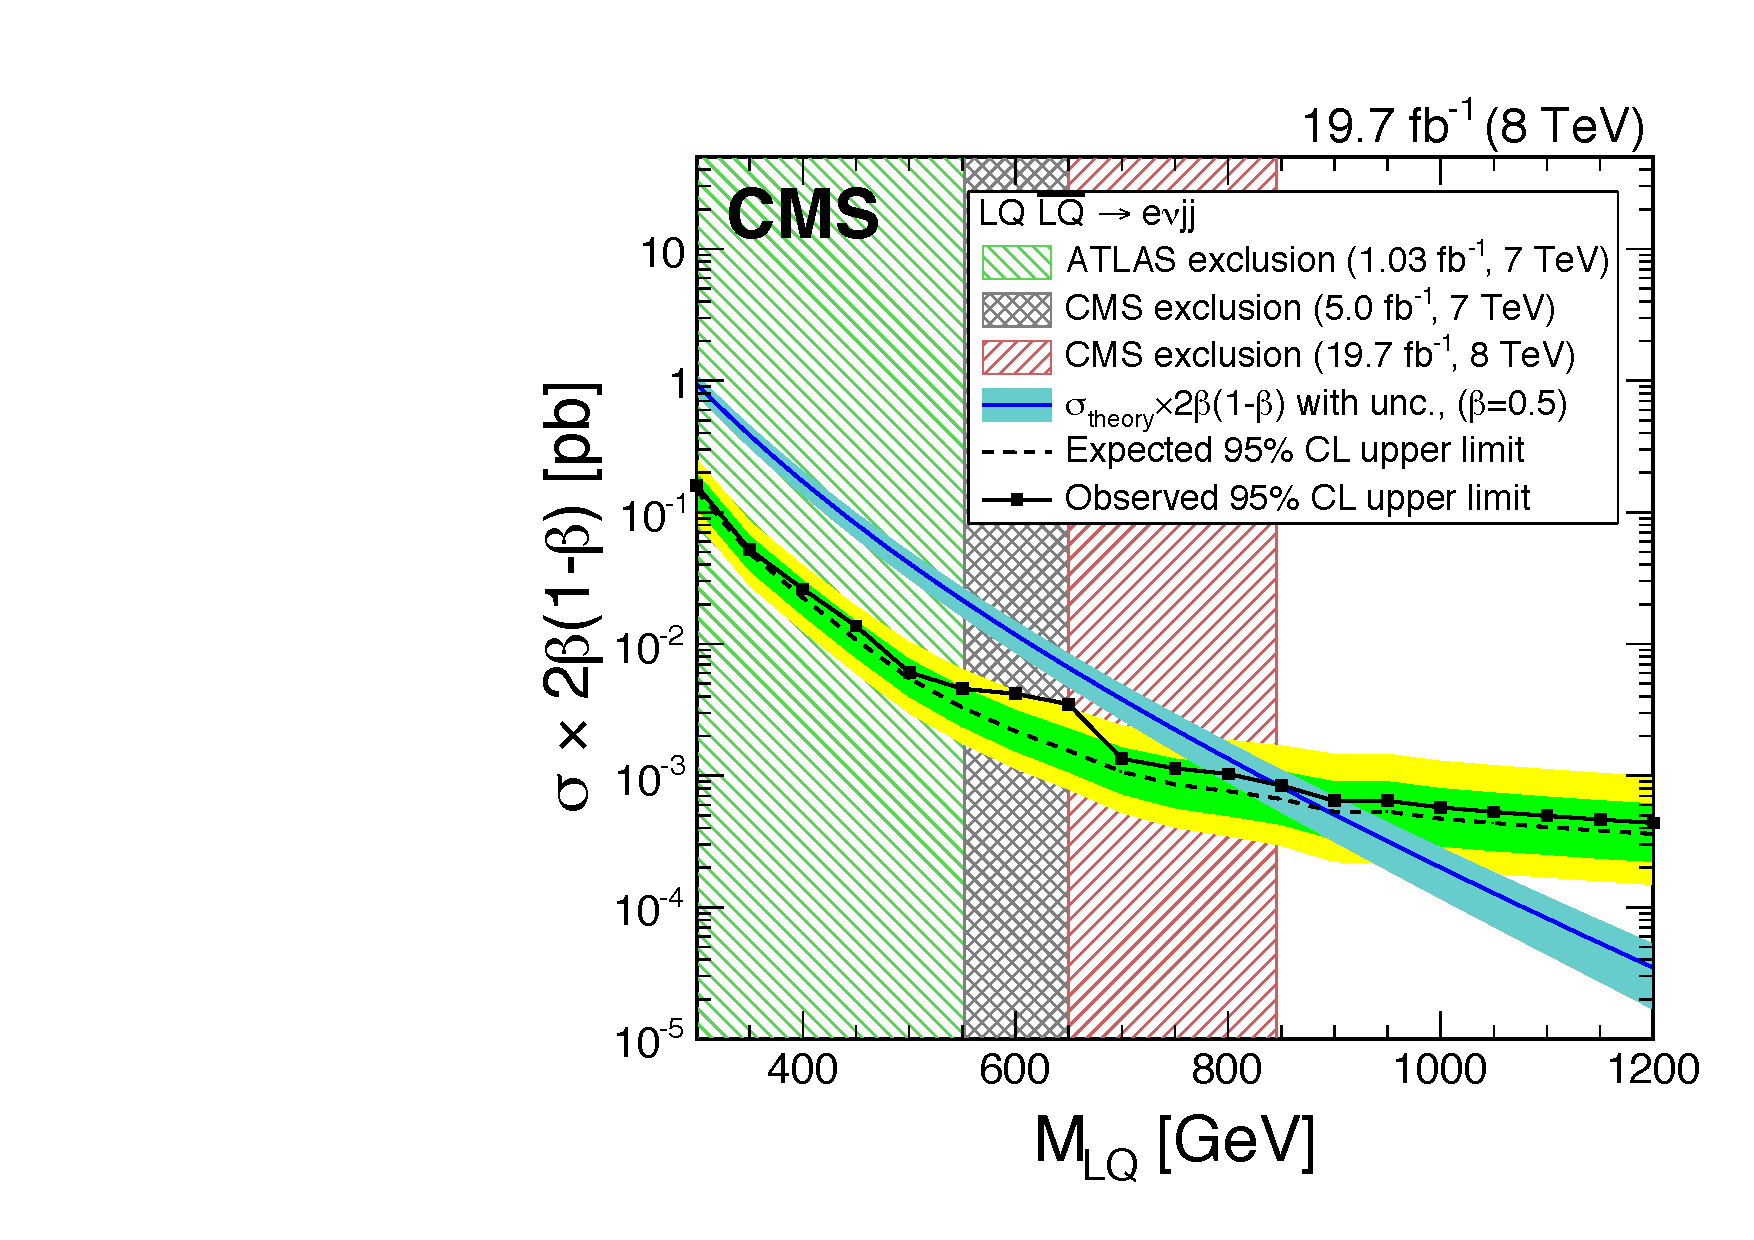
\includegraphics[width=6cm,clip]{CMS-EXO-12-041_Figure_010-b.pdf}
\caption{Left: The $M_{ej}$ distribution in the $e\nu jj$ channel after the
  selection criteria optimized for a LQ mass of 650 GeV have been
  applied. Right: the expected and observed upper limits at 95\% CL on
the LQ pair production cross section times branching ratio as a
function of the first generation LQ mass obtained in the $e\nu jj$ channel.}
\label{LQ1}       % Give a unique label
\end{figure}
%

\subsection{$W_R$ and heavy Majorana neutrinos}

The second analysis is a search for $W_R$ and heavy Majorana
neutrinos~\cite{Khachatryan:2014dka}. These new heavy particles are predicted in
left-right symmetric extensions of the Standard Model. 
The model introduces an additional right-handed SU$_R(2)$ symmetry
group to the SM, which includes heavy charged ($W^{\pm}_R$) and
neutral ($Z_R$) gauge bosons in addition to heavy right-handed
Majorana neutrinos ($N_e$, $N_\mu$, $N_{\tau}$). The latter ones
provide a possible explanation for the mass of SM neutrinos through
the so called {\it see-saw} mechanism.
Figure~\ref{heavyNeutrino} (left) shows a diagram of the production and decay of a
massive $W_R$ gauge boson decaying to an heavy Majorana neutrino.
The final state contains two charged, same-flavour leptons and two jets. In presence of
a signal the invariant mass of the four-body system $M_{\ell\ell jj}$ peaks
at the mass of the $W_R$ boson. Figure~\ref{heavyNeutrino} (right) shows the 
$M_{eejj}$ distribution in data events with two electrons and two jets. An excess is visible at around 2 TeV
corresponding to a local significance of 2.8 standard deviations. 
No excess is observed in the two muons plus two jets channel.
%
\begin{figure}[h]
\centering
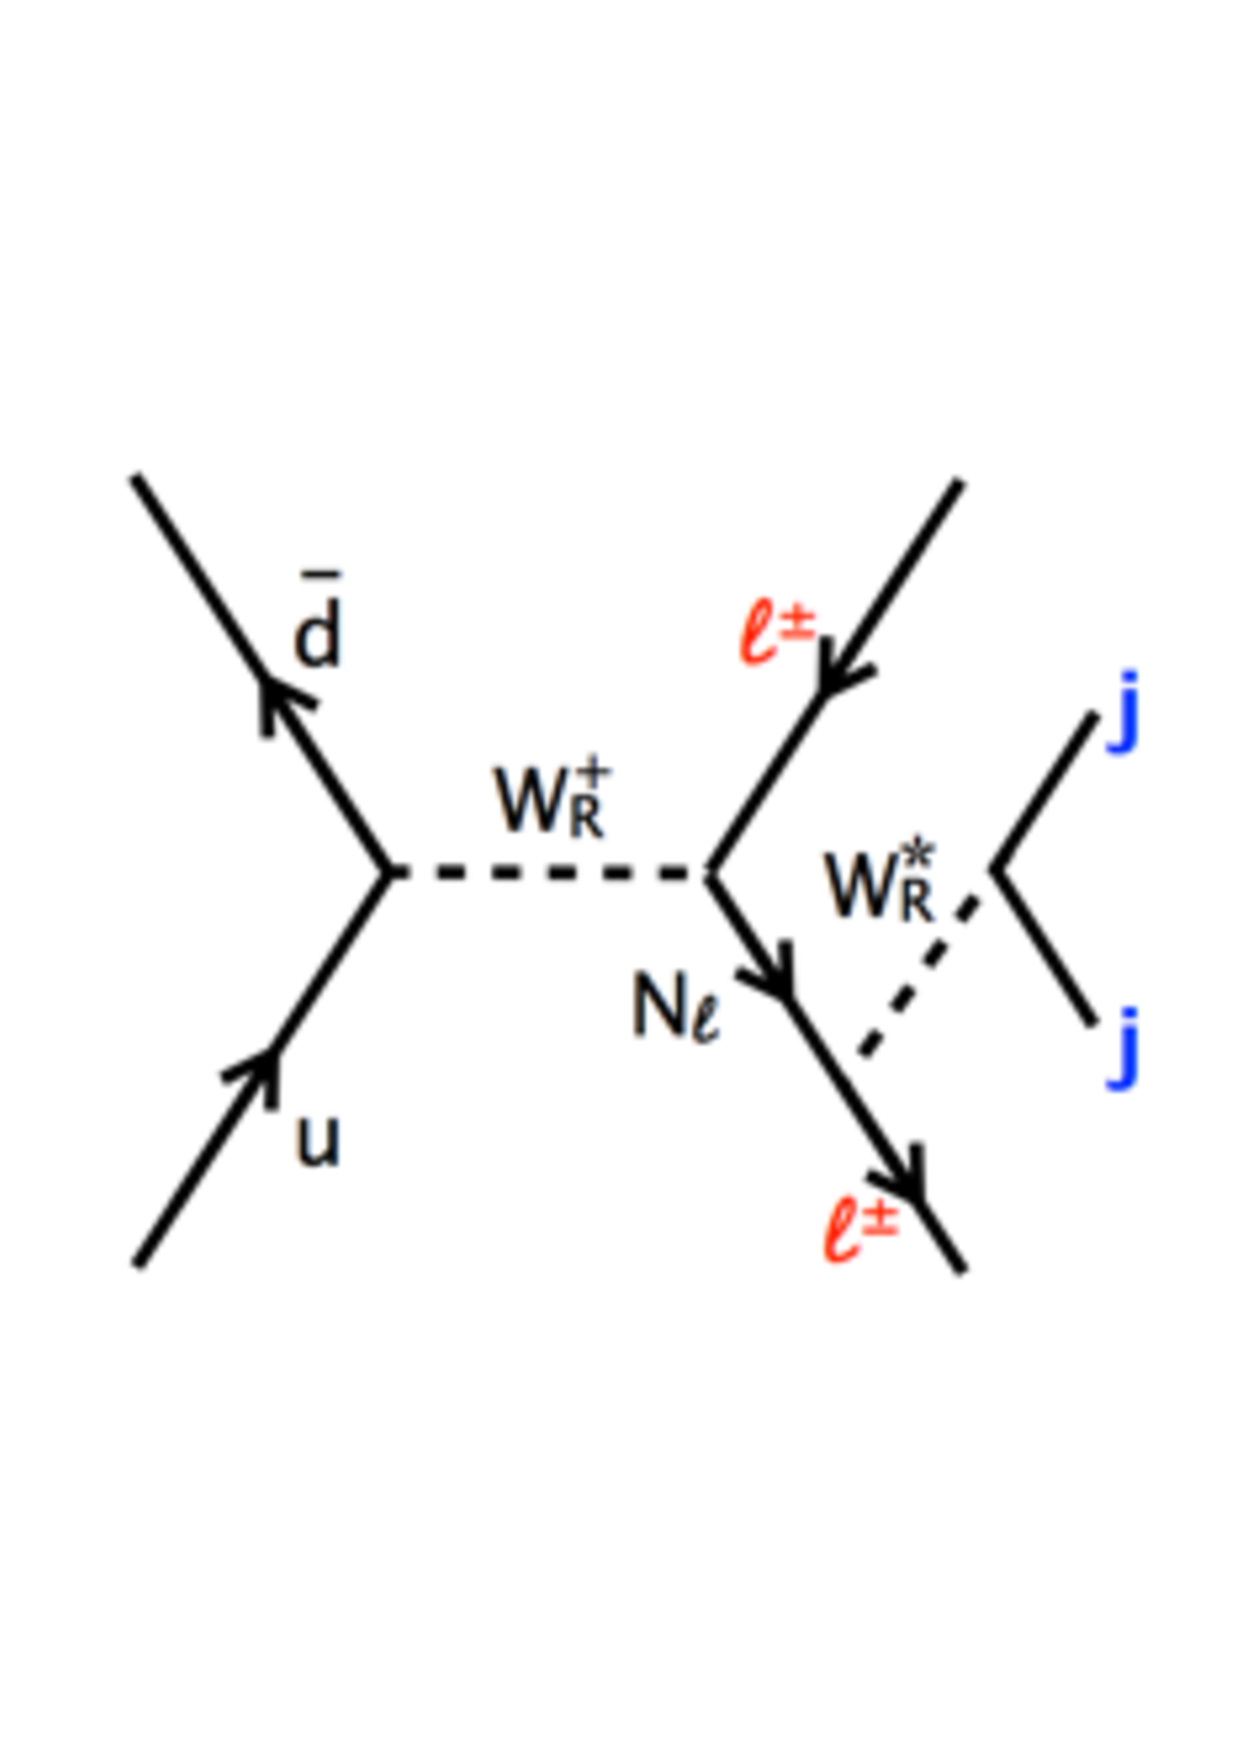
\includegraphics[width=5cm,clip]{WRdiagram.pdf}
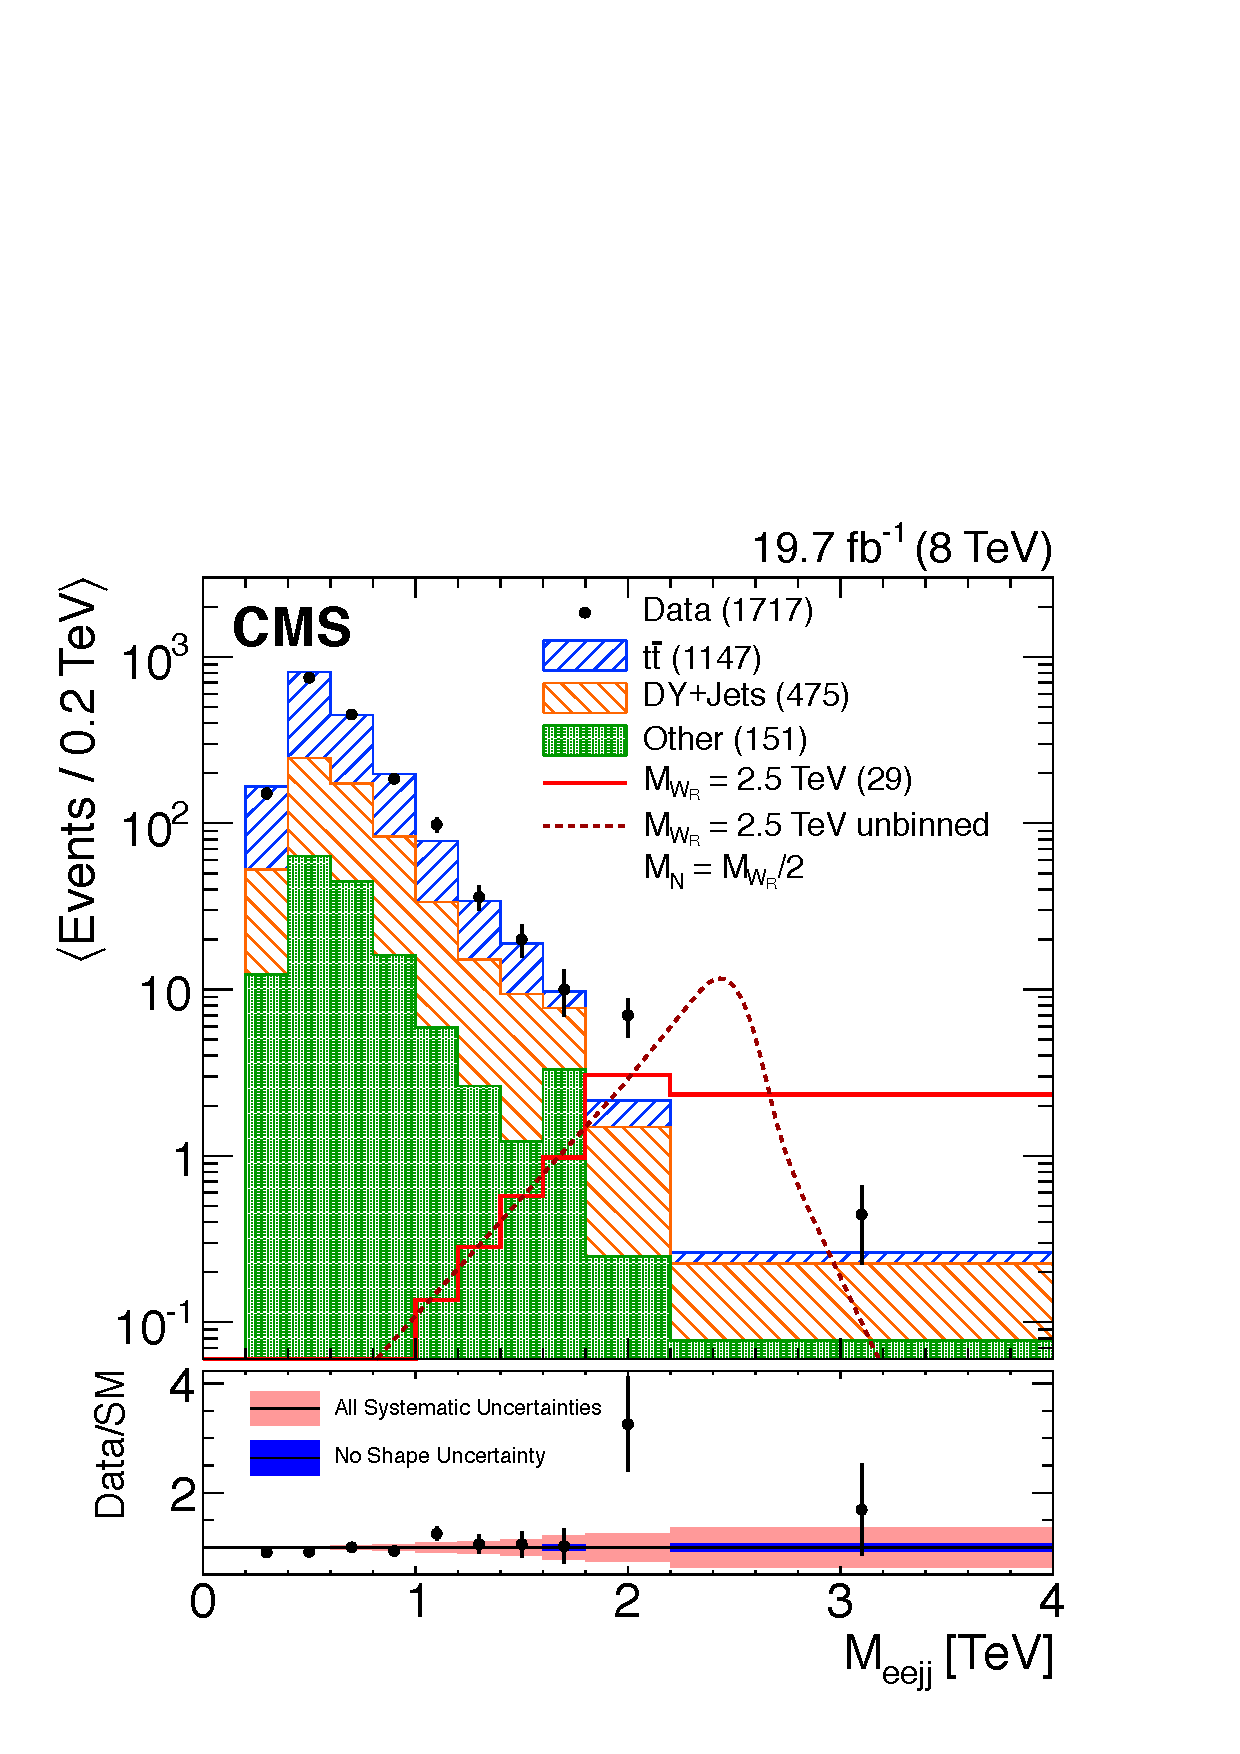
\includegraphics[width=6cm,clip]{CMS-EXO-13-008_Figure_002-a.pdf}
\caption{Left: Diagram of production of $W_R$ and decay to heavy
  Majorana Neutrino. Right: $M_{eejj}$ distribution in events with two electrons
  and two jets after full selection.}
\label{heavyNeutrino}       % Give a unique label
\end{figure}
%

\section{Future prospects}
\label{future}

Searches in jets and leptons+jets final states at CMS are ongoing
using the recent 2016 data.  A datasample of about  40 fb$^{-1}$ should be recorded at $\sqrt{s}=13$~TeV
for both ATLAS and CMS experiments. The sensitivity to new physics of 
the searches presented in this document will improve significantly
compared to the current results thanks to a dataset 20 times larger
than 2015.

At the date of this conference, the two searches 
discussed in Section~\ref{excess} have not being repeated yet at
$\sqrt{s}=13$~TeV neither by ATLAS or CMS experiments.
Although the observed excesses are still compatible with statistical
fluctuations of the background, it is very interesting to see if the
new analyses will confirm the results observed in the 8 TeV data. 
New results from the CMS collaboration are expected in 2017.

%For tables use syntax in table~\ref{tab-1}.
%\begin{table}[h]
%\centering
%\caption{Please write your table caption here}
%\label{tab-1}       % Give a unique label
%% For LaTeX tables you can use
%\begin{tabular}{lll}
%\hline
%first & second & third  \\\hline
%number & number & number \\
%number & number & number \\\hline
%\end{tabular}
%% Or use
%%\vspace*{5cm}  % with the correct table height
%\end{table}


%
% BibTeX or Biber users please use (the style is already called in the class, ensure that the "woc.bst" style is in your local directory)
% \bibliography{name or your bibliography database}
%
% Non-BibTeX users please use
%


\begin{thebibliography}{}
%
% and use \bibitem to create references.
%

%\begin{itemize}
%\item 
%\end{itemize}

\bibitem{EXOpages}
% Format for Journal Reference
http://cms-results.web.cern.ch/cms-results/public-results/publications/EXO/index.html 
http://cms-results.web.cern.ch/cms-results/public-results/preliminary-results/EXO/index.html
% Format for books

\bibitem{Khachatryan:2015dcf} 
  CMS Collaboration,
  ``Search for narrow resonances decaying to dijets in proton-proton collisions at $\sqrt(s) =$ 13 TeV,''
  Phys.\ Rev.\ Lett.\  {\bf 116}, no. 7, 071801 (2016),
  arXiv:1512.01224.

\bibitem{CMS:2012cza} 
  CMS Collaboration,
  ``Search for Narrow Resonances using the Dijet Mass Spectrum in pp Collisions at sqrt s of 7 TeV,''
  CMS-PAS-EXO-11-094.

\bibitem{CMS:2012ooa} 
  CMS Collaboration,
  ``Data Parking and Data Scouting at the CMS Experiment,''
  CMS-DP-2012-022.

\bibitem{Khachatryan:2016ecr} 
  CMS Collaboration,
  ``Search for narrow resonances in dijet final states at $\sqrt(s)=$ 8 TeV with the novel CMS technique of data scouting,''
  Phys.\ Rev.\ Lett.\  {\bf 117}, no. 3, 031802 (2016), 
  arXiv:1604.08907.

\bibitem{Dobrescu:2013coa} 
  B.~A.~Dobrescu and F.~Yu,
  ``Coupling-mass mapping of dijet peak searches,''
  Phys.\ Rev.\ D {\bf 88}, no. 3, 035021 (2013), 
  Erratum: [Phys.\ Rev.\ D {\bf 90}, no. 7, 079901 (2014)], 
  arXiv:1306.2629.

\bibitem{CMS:2016qhm} 
  CMS Collaboration,
  ``Search for pair-production of second-generation scalar leptoquarks
  in pp collisions at $\sqrt{s}=13~\mathrm{TeV}$ with the CMS
  detector,'' CMS-PAS-EXO-16-007.

\bibitem{CMS:2016xxl} 
  CMS Collaboration,
  ``Search for heavy neutrinos and third-generation leptoquarks in final states with two hadronically decaying $\tau$ leptons and two jets in proton-proton collisions at $\sqrt{s} = 13~\mathrm{TeV}$,''
  CMS-PAS-EXO-16-016.

\bibitem{Khachatryan:2015vaa} 
  CMS Collaboration,
  ``Search for pair production of first and second generation leptoquarks in proton-proton collisions at sqrt(s) = 8 TeV,''
  Phys.\ Rev.\ D {\bf 93}, no. 3, 032004 (2016)
  arXiv:1509.03744.

\bibitem{Khachatryan:2014dka} 
  CMS Collaboration,
  ``Search for heavy neutrinos and $\mathrm {W}$ bosons with right-handed couplings in proton-proton collisions at $\sqrt{s} = 8\,\text {TeV} $,''
  Eur.\ Phys.\ J.\ C {\bf 74}, no. 11, 3149 (2014)
  arXiv:1407.3683.

%\bibitem{RefJ}
%% Format for Journal Reference
%Journal Author, Journal \textbf{Volume}, page numbers (year)
%% Format for books
%\bibitem{RefB}
%Book Author, \textit{Book title} (Publisher, place, year) page numbers
%% etc
\end{thebibliography}

\end{document}

% end of file template_ICNFP2015.tex

